\documentclass[14pt]{article}
\usepackage{amsmath}
\usepackage{listings} % For writing code see http://ctan.org/pkg/listings
\usepackage{graphicx}
\usepackage{float}
\usepackage[margin=1.0in]{geometry}
\usepackage{hyperref}
\usepackage{fancyhdr}
\usepackage{natbib}

\bibliographystyle{humannat}

\pagestyle{fancy}

\title{Choosing the number of coefficients needed in a BFE.}
\author{Nico Garavito-Camargo}


\date{}
\begin{document}
\maketitle

\section*{Computing coefficients and the gravitational potential
energy}

Following the notation in \cite{Lowing11}, the coefficients in a BFE around a
Hernquist profile are:

\begin{equation}\label{eq:coeff}
  \begin{aligned}
    S_{nlm} = (2-\delta_{m0})\tilde{A}_{nl} \sum_k m_k
  \Phi_{nl}(r_k)Y_{lm}(\theta_k) cos\ m\phi_k \\
    T_{nlm} = (2-\delta_{m0})\tilde{A}_{nl} \sum_k m_k 
  \Phi_{nl}(r_k)Y_{lm}(\theta_k) sin\ m\phi_k 
  \end{aligned}
\end{equation}

With these coefficients the density and potential are found to be:


\begin{equation}\label{eq:rho}
  \rho(r, \theta, \phi) = \sum_{n} \sum_l \sum_m Y_{lm}(\theta) \rho_{nl}(r)
  \left[ S_{nlm} cos\ m \phi + T_{nlm} sin\ m\phi \right]
\end{equation}


\begin{equation}\label{eq:phi}
  \Phi(r, \theta, \phi) = \sum_{n} \sum_l \sum_m Y_{lm}(\theta) \Phi_{nl}(r)
  \left[ S_{nlm} cos\ m\phi + T_{nlm} sin\ m \phi \right]
\end{equation}

A complete derivation of Equations \ref{eq:coeff}, \ref{eq:rho}, \ref{eq:phi}
are found in the Appendix \ref{sec:appendix}.

The total gravitational potential energy of the system is:

\begin{equation}\label{eq:energy}
  U = \dfrac{1}{2} \int_V \rho(r, \theta, \phi)\Phi(r,\theta, \phi)^{*} d^3
  \textbf{r} =  \dfrac{1}{2}\sum_{nlm} \frac{S_{nlm}^2 +
  T_{nlm}^2}{\tilde{A}_{nl}} 
\end{equation}

Where the term on the right hand side was derived using orthogonal properties of
the Spherical harmonics see appendix \ref{sec:appendix} for details. 



\section{Computation of the expansion coefficients and the gravitational
potential energy in Hernquist halos}
\subsection{Spherical Halo:}

Figure \ref{fig:coeff_hernquist} shows the value of the coefficients $S_{nlm}$
defined in Equation \ref{eq:coeff} for a Dark
Matter halo with a Hernquist profile and scale length of $a= 40 kpc$. The left
panel on Figure \ref{fig:coeff_hernquist} shows the value of the
coefficients as a function of $n$. The first and the second terms are the
only coefficients that have a noticeable contribution. On the right panel, the
coefficients are shown as a function of $l$, here we see how the amplitude of
the coefficients increase exponentially with $l$. 

\begin{figure}[H]
  \centering
  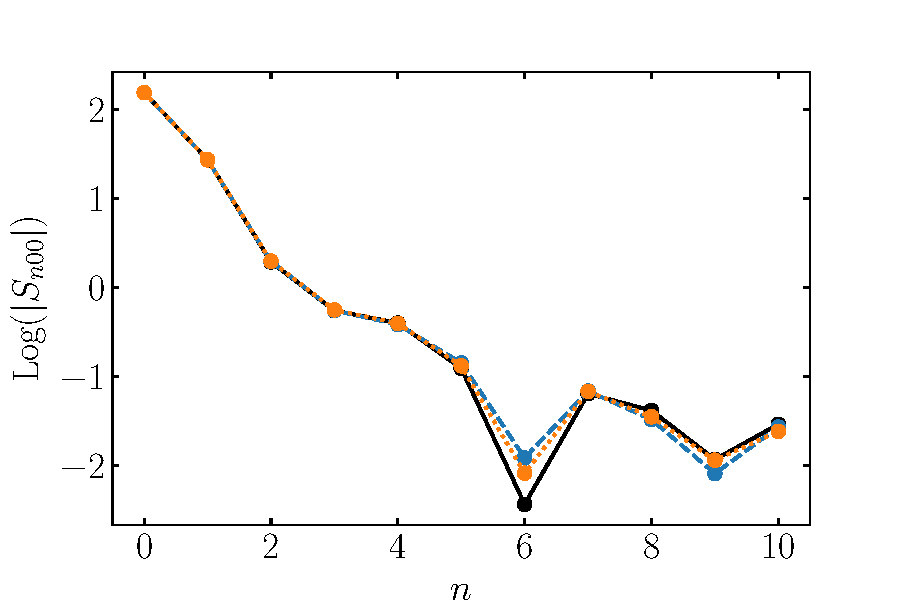
\includegraphics[scale=0.5]{../code/S_n_henrquist.pdf}
  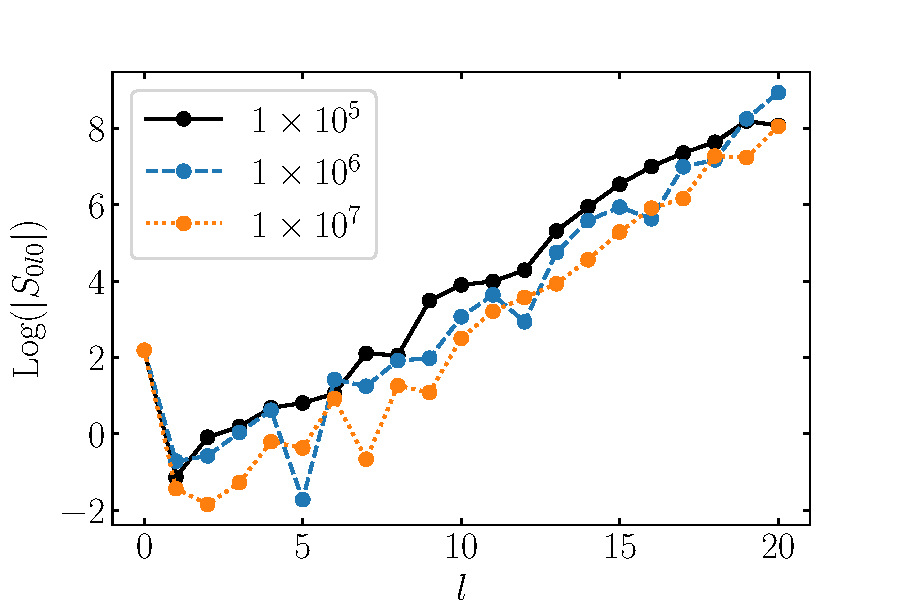
\includegraphics[scale=0.5]{../code/S_l_henrquist.pdf}
  \caption{Coefficients computed using equation \label{eq:coeff} as a function
  of $n$ (left) and $l$ (right). The amplitude of the coefficients increase
  exponentially with $l$} \label{fig:coeff_hernquist}
\end{figure}

Figure \ref{fig:spherical_energy} shows the energy terms from Equation
\ref{eq:energy}. The first 

\begin{figure}[H]
  \centering
  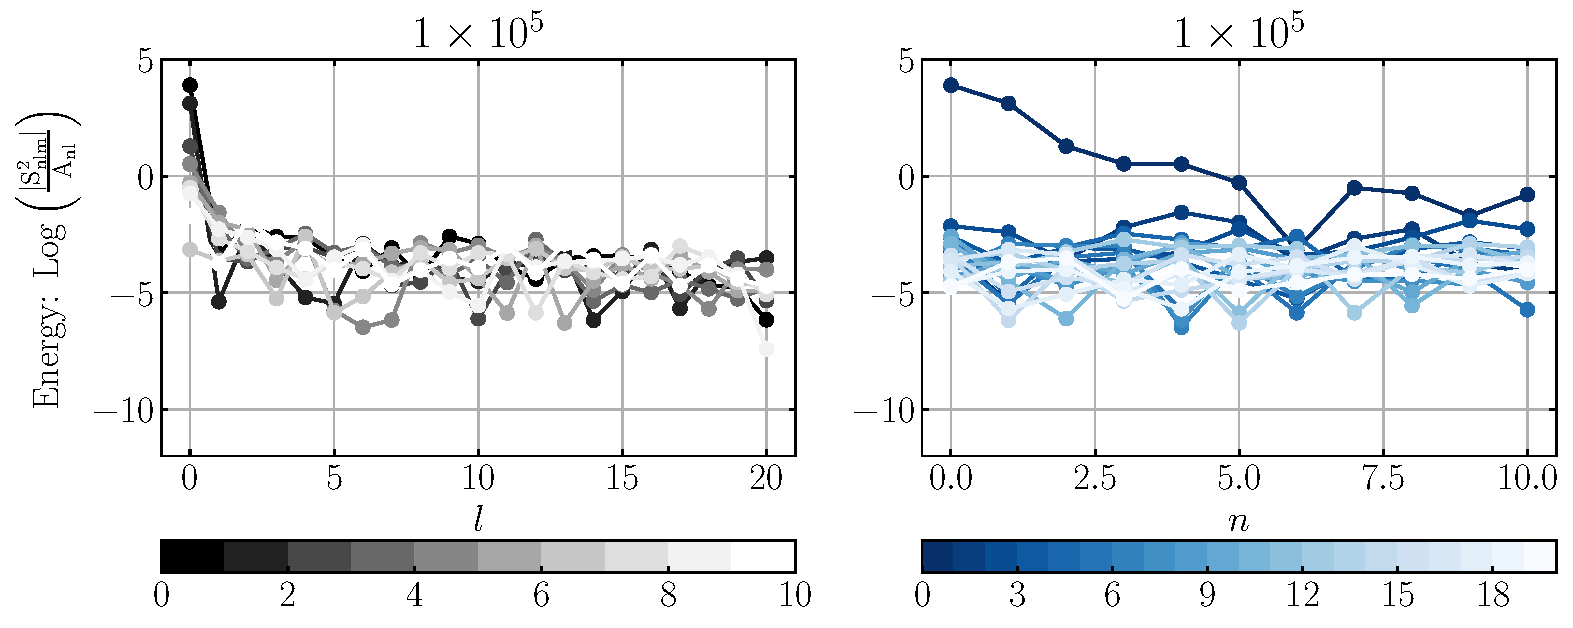
\includegraphics[scale=0.5]{../code/energy_terms_hern_a_40_1E5.pdf}
  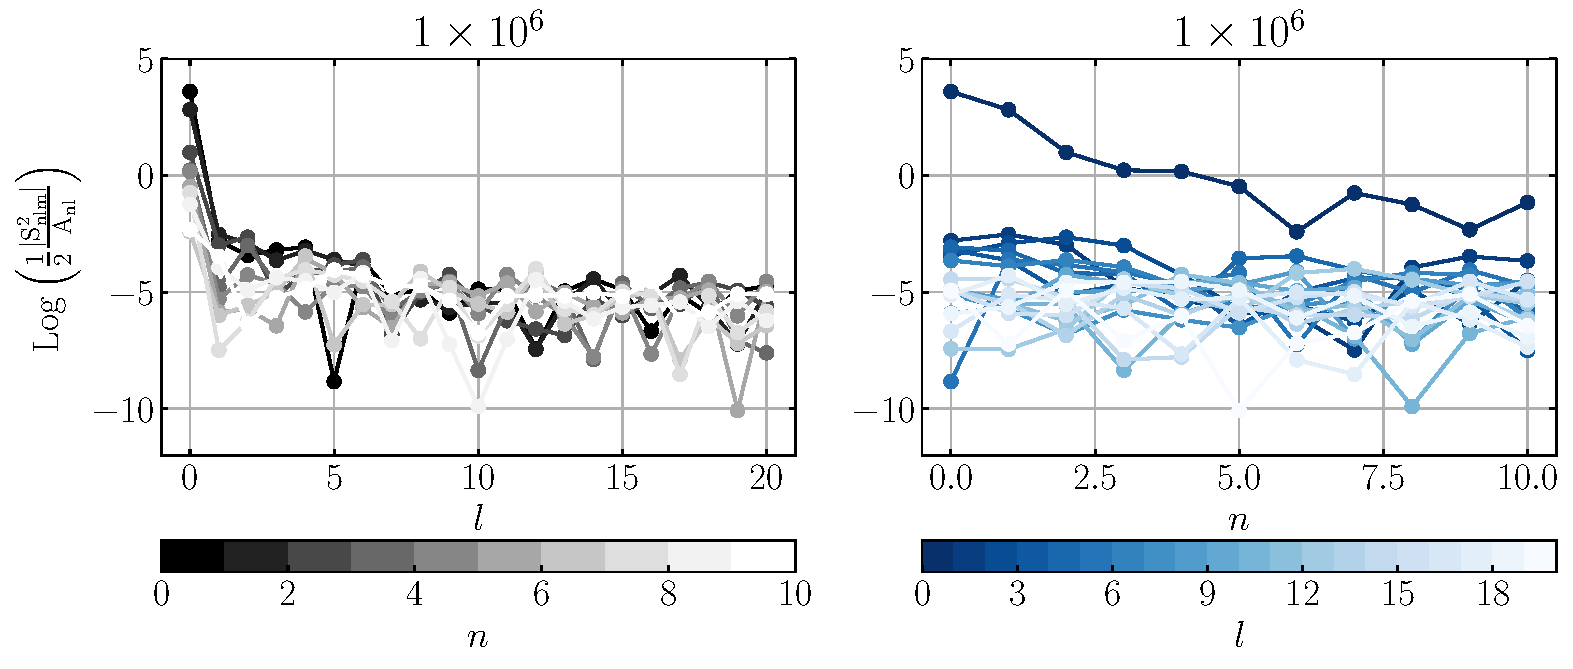
\includegraphics[scale=0.5]{../code/energy_terms_hern_a_40_1E6.pdf}
  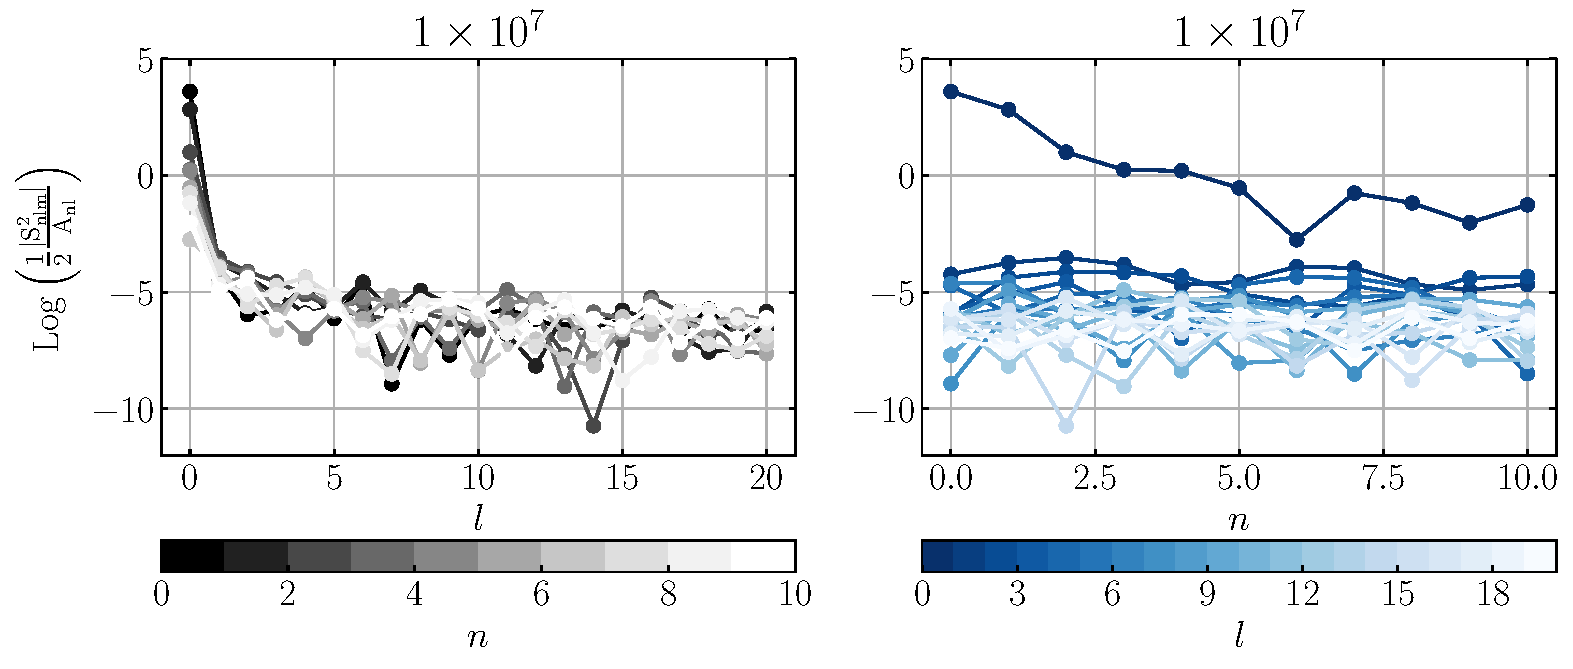
\includegraphics[scale=0.5]{../code/energy_terms_hern_a_40_1E7.pdf}
  \caption{Terms on the potential energy  contribution}\label{fig:spherical_energy}
\end{figure}

\subsection{Oblate halo}

If one repeats the computations of the coefficients and the energy terms for a
Hernquist oblate halo with axis ratios of XX one finds that the coefficients
with $l=2,4,6$ have higher amplitudes when compare to the spherical case as shown
in Figure \ref{fig:oblate_coeff}. 


\begin{figure}[H]
  \centering
  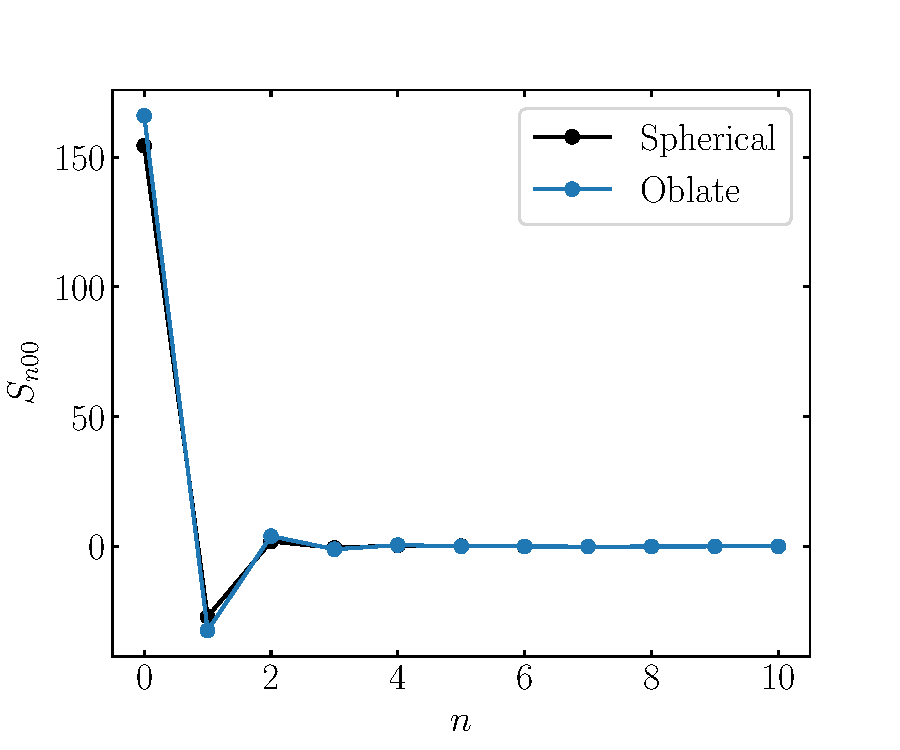
\includegraphics[scale=0.5]{../code/S_n_henrquist_oblate.pdf}
  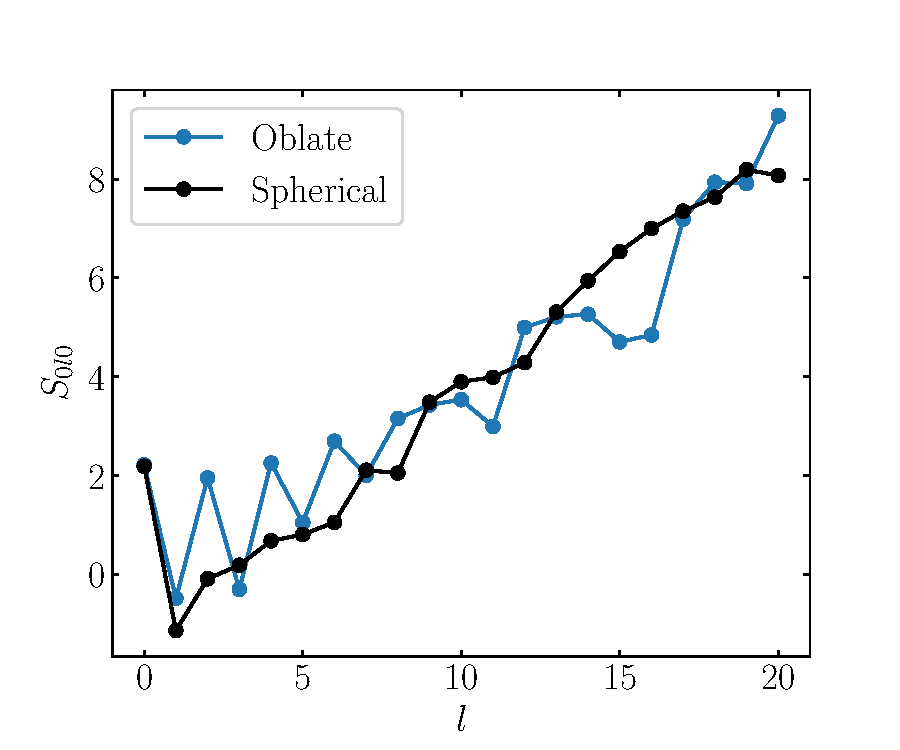
\includegraphics[scale=0.5]{../code/S_l_henrquist_oblate.pdf}
  \caption{Expansion coefficients computed using equation \label{eq:coefficients}}\label{fig:oblate_coeff}
\end{figure}

The corresponding energy terms are 

\begin{figure}[H]
  \centering
  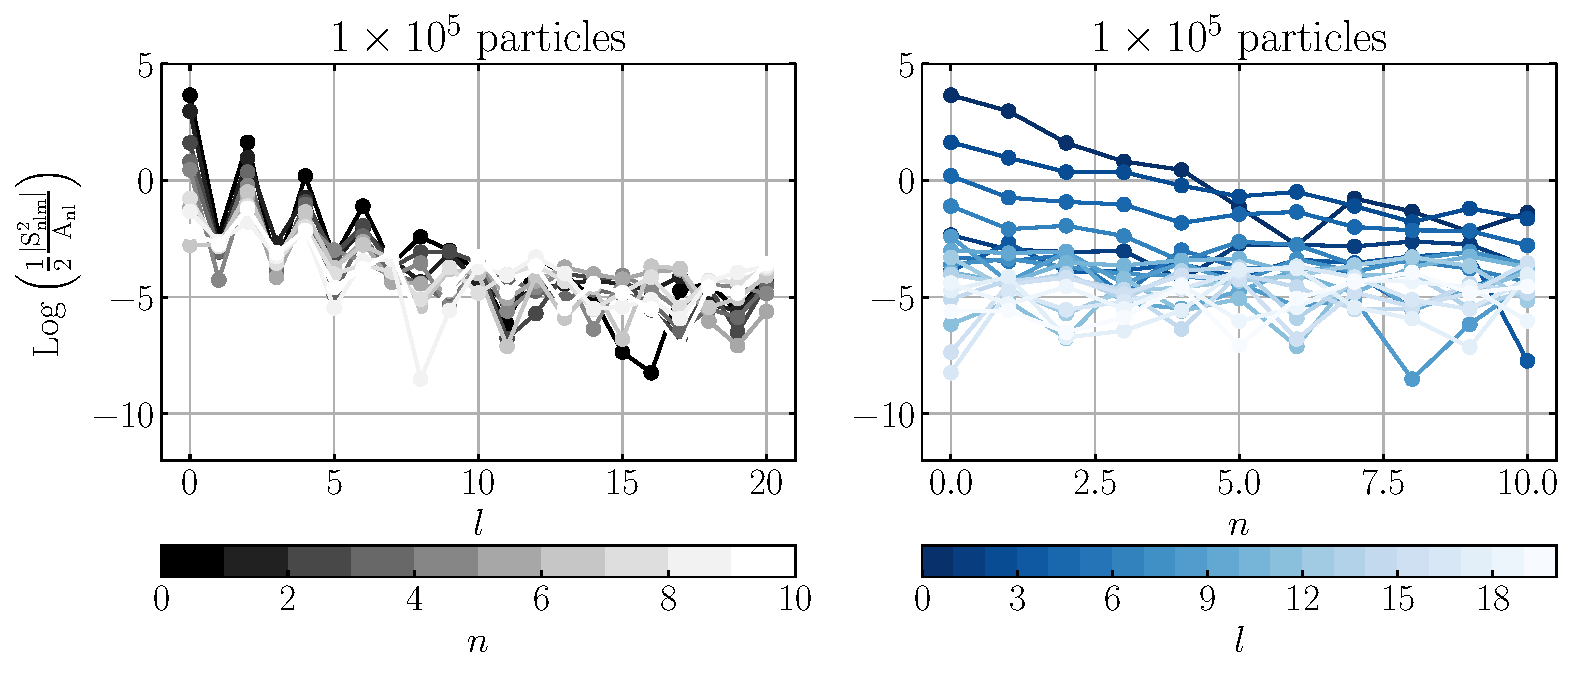
\includegraphics[scale=0.5]{../code/energy_terms_oblate_hern_a_40_1E5.pdf}
  \caption{Terms on the potential energy contribution}
\end{figure}




\textbf{Conclusion:} The coefficients naturally increase as a function of $l$
even if the underlying halo is is Hernquist halo. However, the contribution to 
the potential and to the energy terms, as shown in the right panel of Figure 
\ref{fig:coeff_hernquist}, is negligible. 


Apply energy cut to identify coefficients.

Make a proposal of how to combine this with variance a PCA. 

Next steps: -PCA? - Trying out how the simulations look like. Can I see a really
obvious term as a function of resoluion.

\bibliography{references}


\appendix


\section*{Appendix: A review of the BFE formalism:}\label{sec:appendix}

In this document we will follow the notation presented \cite{Lowing11}. Table
\ref{tab:conversion} shows the conversion between the notation used in \cite{Hernquist92} and
in \cite{Lowing11}.

\begin{table}[h]
  \centering
  \begin{tabular}{c  c}
    \hline
    \hline
    \cite{Hernquist92} notation & \cite{Lowing11} notation \\
    \hline
    $A_{nlm}$ & $S_{nlm} cos\ m\phi + T_{nlm}sin\ m\phi $\\
    $I_{nl} = \frac{1}{\tilde{A}_{nl}}$ & $\frac{1}{\tilde{A}_{nl}}$\\
    $K_{nl}$ & $K_{nl}$ \\
    $\tilde{\rho}_{nl}$ & $\rho_{nl}$\\
    $\tilde{\Phi}_{nl}$ & $\Phi_{nl}$\\
    \hline
    \hline
  \end{tabular}
  \caption{Notation conversion between \cite{Hernquist92} and the
  \cite{Lowing11} works}\label{tab:conversion}
\end{table}



The main idea of the BFE formalism is to expand the potential and density in
angular and radial functions. 


\begin{equation}
    \rho(r, \theta, \phi) = \sum_{nlm} A_{nlm}\rho_{nlm}(r, \theta, \phi)
\end{equation}

\begin{equation}
    \Phi(r, \theta, \phi) = \sum_{nlm} A_{nlm}\Phi_{nlm}(r, \theta, \phi)
\end{equation}

Where $A_{nlm}$ are the coefficients of the expansion. The angular and radial
dependencies can be separated follows:


\begin{equation}\label{eq:potdens_nlm}
  \begin{aligned}
  \Phi_{nlm}(r, \theta, \phi) = \Phi_{nl}(r)Y_{lm}(\theta, \phi)\\ 
  \rho_{nlm}(r, \theta, \phi) = \rho_{nl}(r)Y_{lm}(\theta, \phi) 
  \end{aligned}
\end{equation}


Where $Y_{lm}(\theta,\phi)$ are the spherical harmonics. The radial component
is expended around a Hernquist profile multiplied by the Ultraspherical
polynomials $C_{n}(\xi)$.


\begin{equation}
  \Phi_{nl}(r) = - \dfrac{r^l}{r(1+r)^{2l+3}}C_{n}^{2l+3/2}(\xi)\sqrt{4\pi}
\end{equation}

\begin{equation}
  \rho_{nl}(r) = \dfrac{K_{nl}}{2\pi}\dfrac{r^l}{(1+r)^{2l+1}}C_{n}^{2l+3/2}(\xi)\sqrt{4\pi}
\end{equation}


Where $K_{nl}$ is defined as:

\begin{equation}
    K_{nl}=\dfrac{1}{2}n(n+4l+3) +(l+1)(2l+1)
\end{equation}

The real form of equation \ref{eq:potdens_nlm} takes the form: 

\begin{equation}
  \rho(r, \theta, \phi) = \sum_{n} \sum_l \sum_m Y_{lm}(\theta) \rho_{nl}(r)
  \left[ S_{nlm} cos\ m \phi + T_{nlm} sin m\ \phi \right]
\end{equation}


\begin{equation}
  \Phi(r, \theta, \phi) = \sum_{n} \sum_l \sum_m Y_{lm}(\theta) \Phi_{nl}(r)
  \left[ S_{nlm} cos\ m\phi + T_{nlm} sin\ m \phi \right]
\end{equation}


The coefficients can be computed using the orthonormal properties of the
Spherical harmonics and the Ultraspherical polynomials this is:

\begin{equation}\label{eq:energy}
  I_{nlm}^{n'l'm'} = \int_V \rho_{nlm} \Phi_{n'l'm'}^*  d\textbf{r} = \tilde{A}_{nl} \delta_{nn'}
  \delta_{ll'} \delta_{mm'} 
\end{equation}

Where $\tilde{A}_{nl}$ is found to be:

\begin{equation}
    \tilde{A}_{nl} = - \frac{1}{K_{nl}}\frac{2^{8l+6}}{4\pi}\frac{n!(n+2l+3/2)[\Gamma(2l+3/2)]^2}{\Gamma(n+4l+3)}
\end{equation}

With these relations the coefficients can be derived as follows:

\begin{equation}\label{eq:coefficients}
  I_{nlm} = \int_V \rho(r) \Phi_{nlm} d\textbf{r} = 
\end{equation}


\begin{equation}
  \begin{aligned}
    S_{nlm} = (2-\delta_{m0})\tilde{A}_{nl} \sum_k m_k
  \Phi_{nl}(r_k)Y_{lm}(\theta_k) cos\ m\phi_k \\
    T_{nlm} = (2-\delta_{m0})\tilde{A}_{nl} \sum_k m_k 
  \Phi_{nl}(r_k)Y_{lm}(\theta_k) sin\ m\phi_k 
  \end{aligned}
\end{equation}


With these results we can compute the total gravitational energy of the system
as:

\begin{equation}
  U = \dfrac{1}{2} \int_V \rho(r)\Phi(r)^{*} = \int_v  \sum_{nlm} A_{nlm}^2 \rho_{nlm}(r,
  \theta, \phi) \phi_{nlm}(r, \theta, \phi) = \sum_{nlm}
  \frac{A_{n'l'm'}^2}{\tilde{A}_{nl}}
  \delta_{nn'}\delta_{ll'}\delta_{mm'} 
\end{equation}

\begin{equation}
  U = \dfrac{1}{2}\sum_{nlm} \frac{A_{n'l'm'}^2}{\tilde{A}_{n'l'}} = \sum_{nlm} U_{n'l'm'}
\end{equation}




\end{document}
